\newpage
\section{Implementation, Room module}
The room module is implemented on a ATM328P, the code is implemented using the Arduino toolchain.
The tasks of the module are implemented as pseudo-periodical tasks using the \textit{timer0} to check the activation time of each task branch.

\begin{figure}[h]
	\centering
	\begin{subfigure}{0.4\textwidth} % width of left subfigure
		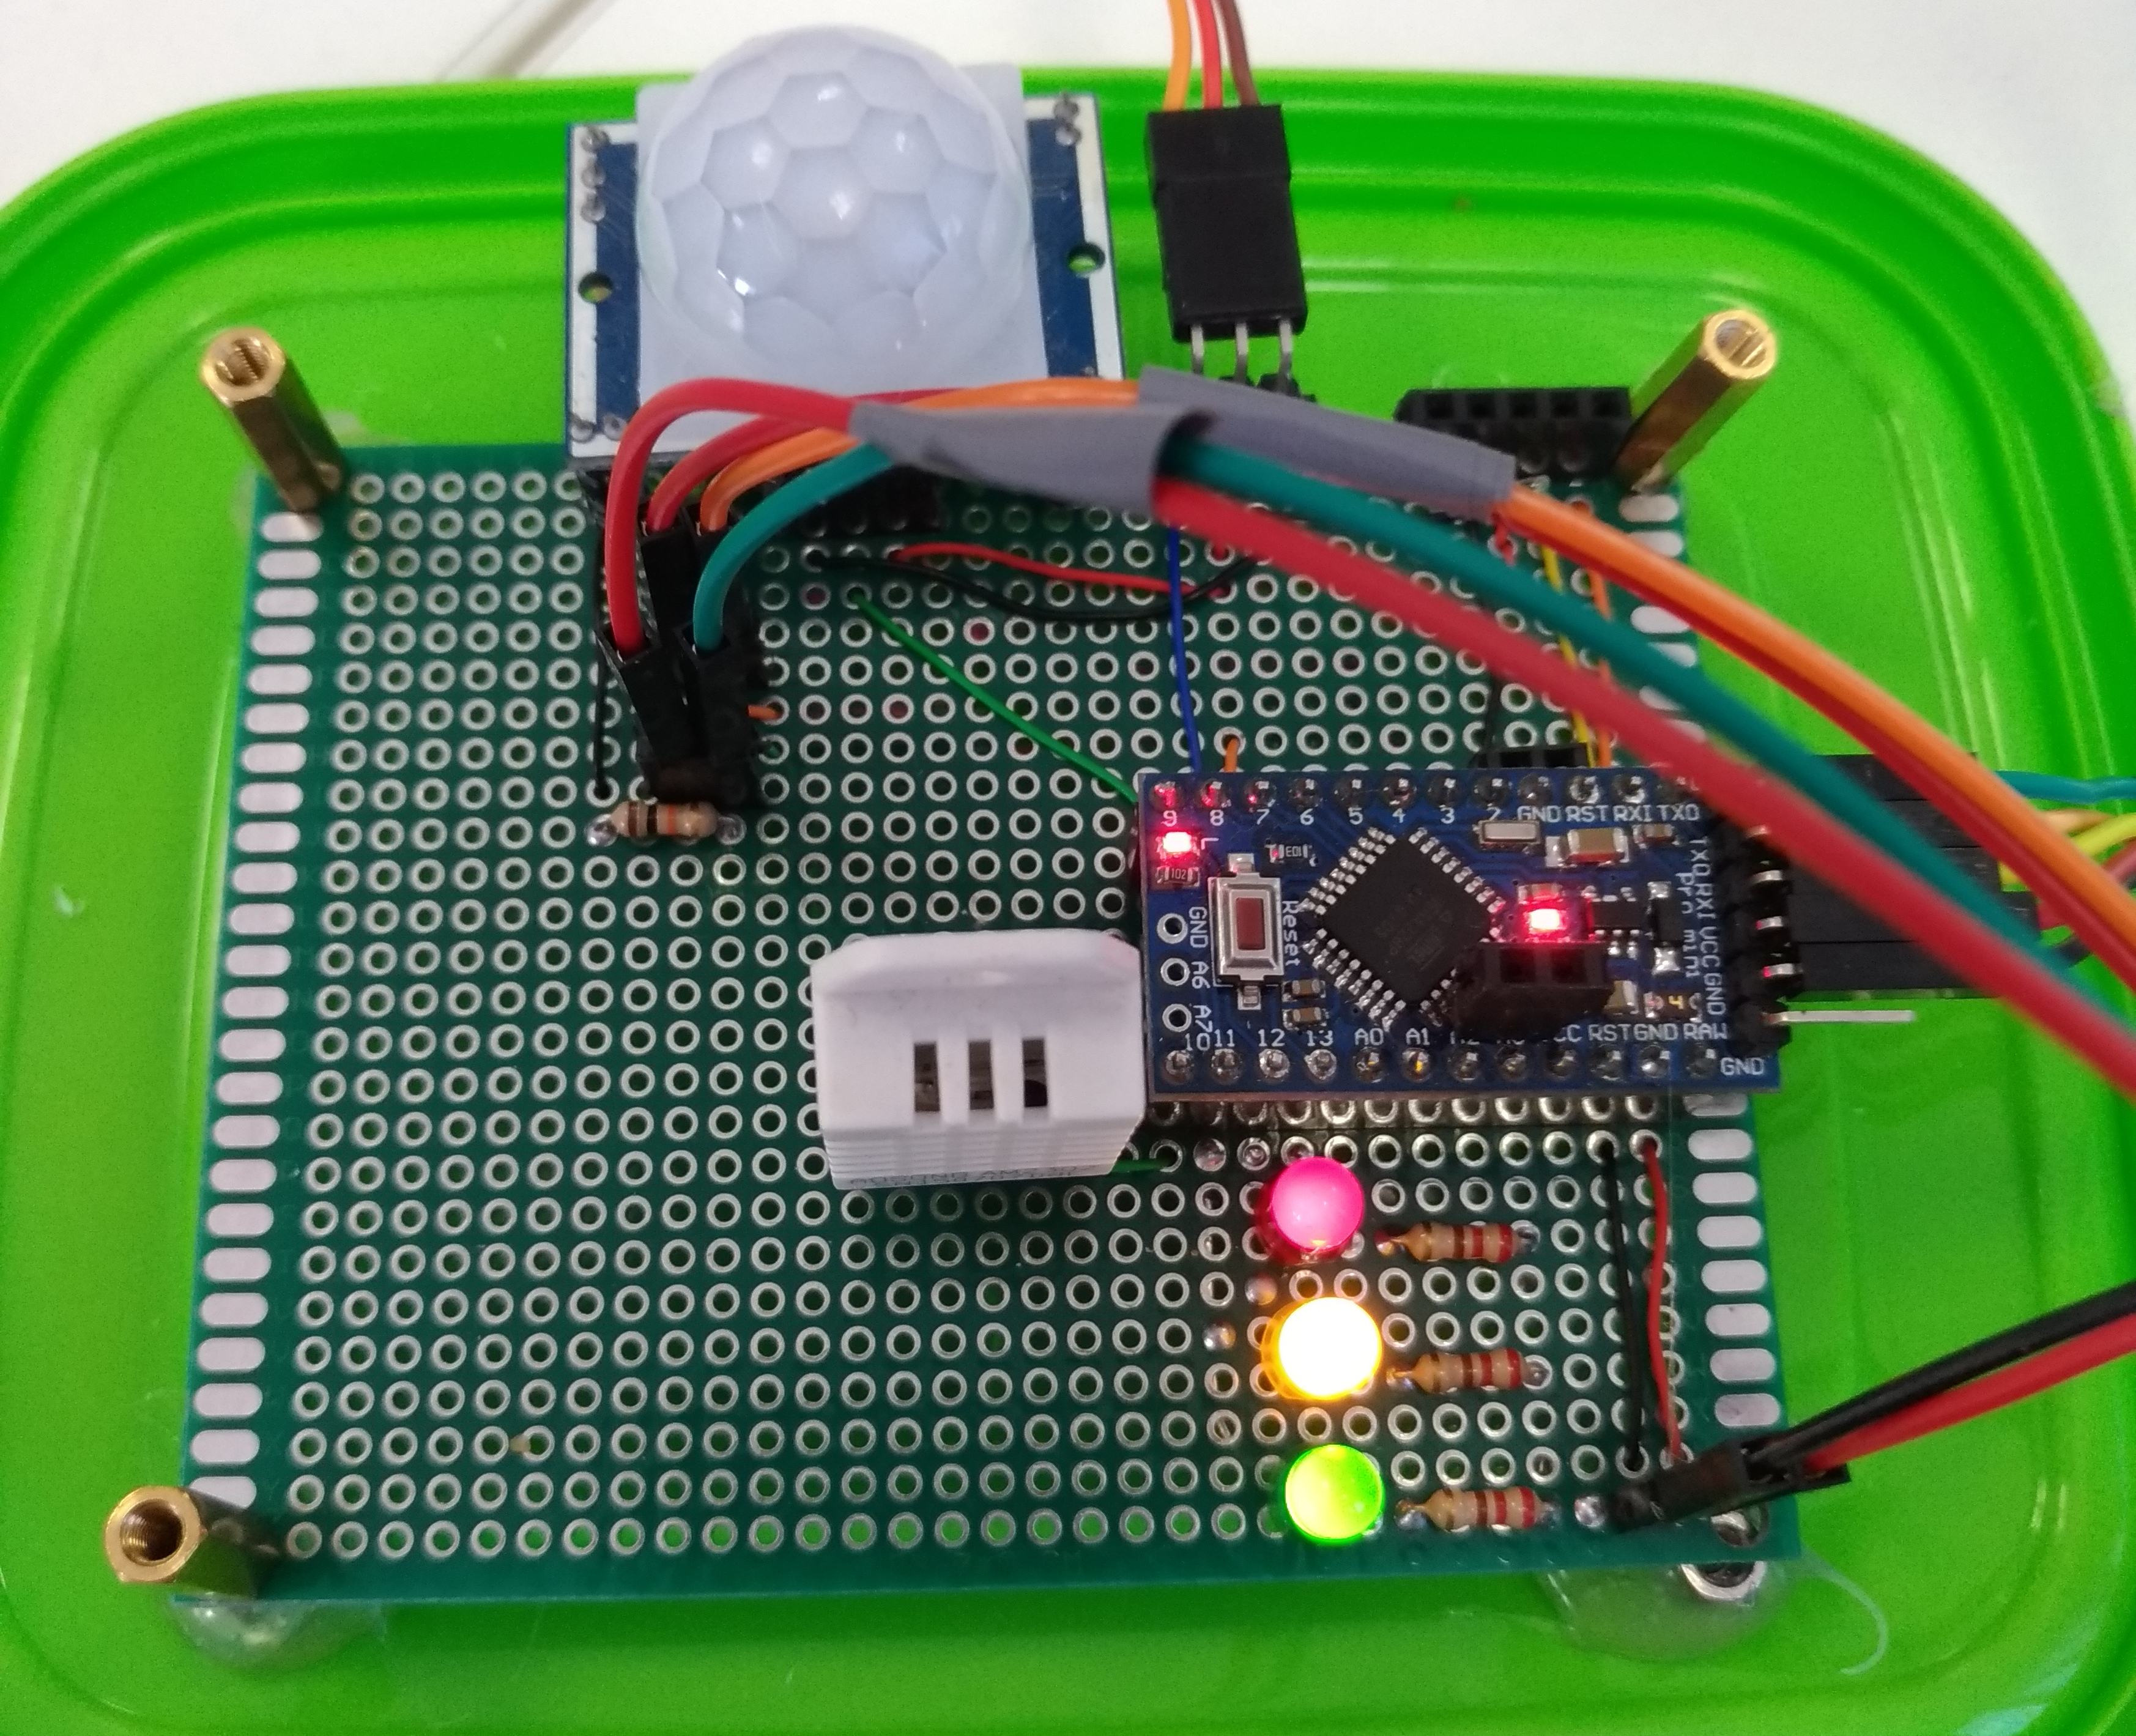
\includegraphics[width=4cm,keepaspectratio]{img/room_board}
		\caption{Room module}
		\label{fig:room_module}
		\end{subfigure}
	\vspace{1em} % here you can insert horizontal or vertical space
	\begin{subfigure}{0.4\textwidth} % width of right subfigure
		
\includegraphics[width=4cm,keepaspectratio]{img/valve}
		\caption{Valve}
		\label{fig:valve}
	\end{subfigure}
\end{figure}


The module is composed by:
\begin{itemize}
	\item Arduino pro mini, Atmega328P (8MHz, 3.3v logic)
	\item DHT22 Temperature and Humidity sensor
	\item PIR motion sensor
	\item Red led
	\item Green led
	\item Yellow led
	\item Servo Motor tower pro SG90
	\item 2 switch to check the open and closed position of the valve
\end{itemize}

\subsection{Components description}
\subsubsection{ServoMotor}
	\begin{figure}[h]
		\centering
		\begin{subfigure}{0.4\textwidth} % width of left subfigure
			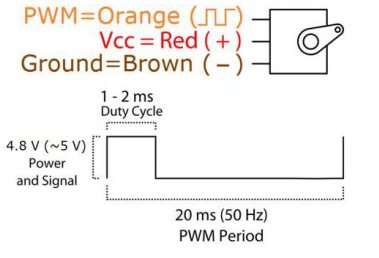
\includegraphics[width=4cm,keepaspectratio]{img/servo_signal}
			\end{subfigure}
		\vspace{1em} % here you can insert horizontal or vertical space
		\begin{subfigure}{0.4\textwidth} % width of right subfigure
			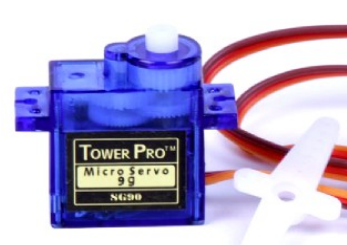
\includegraphics[width=4cm,keepaspectratio]{img/servomotor}
		\end{subfigure}
		\caption{Servo Motor}
		\label{fig:ServoMotor}
	\end{figure}

	The chosen ServoMotor is a Tower Pro SG90 reported in \ref{fig:ServoMotor},
	As reported in the \ref{fig:ServoMotor}, the signal used to move the servomotor in the correct position is a PWM and the duty-cycle describe the position that the motor has to maintain.
	The signal to control the motor position is managed by the Servo library using the \textbf{timer1} a 16-bit timer.
	The digital circuit inside the servomotor will adjust the position of the rotor using a potentiometer attached to that.
	In the following table are reported	the characteristics of the servomotor:
	\begin{center}
		\begin{tabular}{||l | l | l||} 
			\hline
			Voltage(V) & 4.8 - 6 \\ 
			\hline
			Torque(Kg-cm) & 2.5 \\
			\hline
			Speed(sec) & 0.1 \\
			\hline
			Weight(g) & 14.7 \\
			\hline
		\end{tabular}
	\end{center}

\subsubsection{Valve position switches}
\begin{figure}[h]
	\centering
	
\includegraphics[width=6cm,keepaspectratio]{img/valve}
	\caption{Discovery board wiring}
	\label{fig:valve}
\end{figure}
In order to check the position of the valve, two switches are fixed in the open and closed position.
During the \textit{init\_valve} phase the position in degree is saved in order to adjust the possible positions of the valve.
Whenever the valve goes in one of these positions a check is done using the correct switch.	

\subsubsection{Temperature-Humidity Sensor}
The chosen sensor is a DHT22 that is perfect to work in closed environment, 
a pull-up resistor, connecting the data pin to VCC, is used in order to mantain the line clear when no one is transmitting.
The sensor has a dedicated one-wire communication protocol implemented by the DHT adafruit library.
\begin{center}
	\begin{tabular}{||l | l||} 
		\hline
		Voltage(V) & 3 - 5 \\ 
		\hline
		Current(mA) & 2.5 \\
		\hline
		Humidity(\%) & 0 - 100 \\
		\hline
		Humidity Accuracy(\%) & 2 - 5 \\
		\hline
		Temperature(C\degree) & -40 - 80 \\
		\hline
		Temperature Accuracy(C\degree) & +/- 0.5 \\
		\hline
		Sampling rate(Hz) & 0.5 \\
		\hline
	\end{tabular}
\end{center}


\subsection{Wiring}
	\begin{figure}[h]
		\centering
		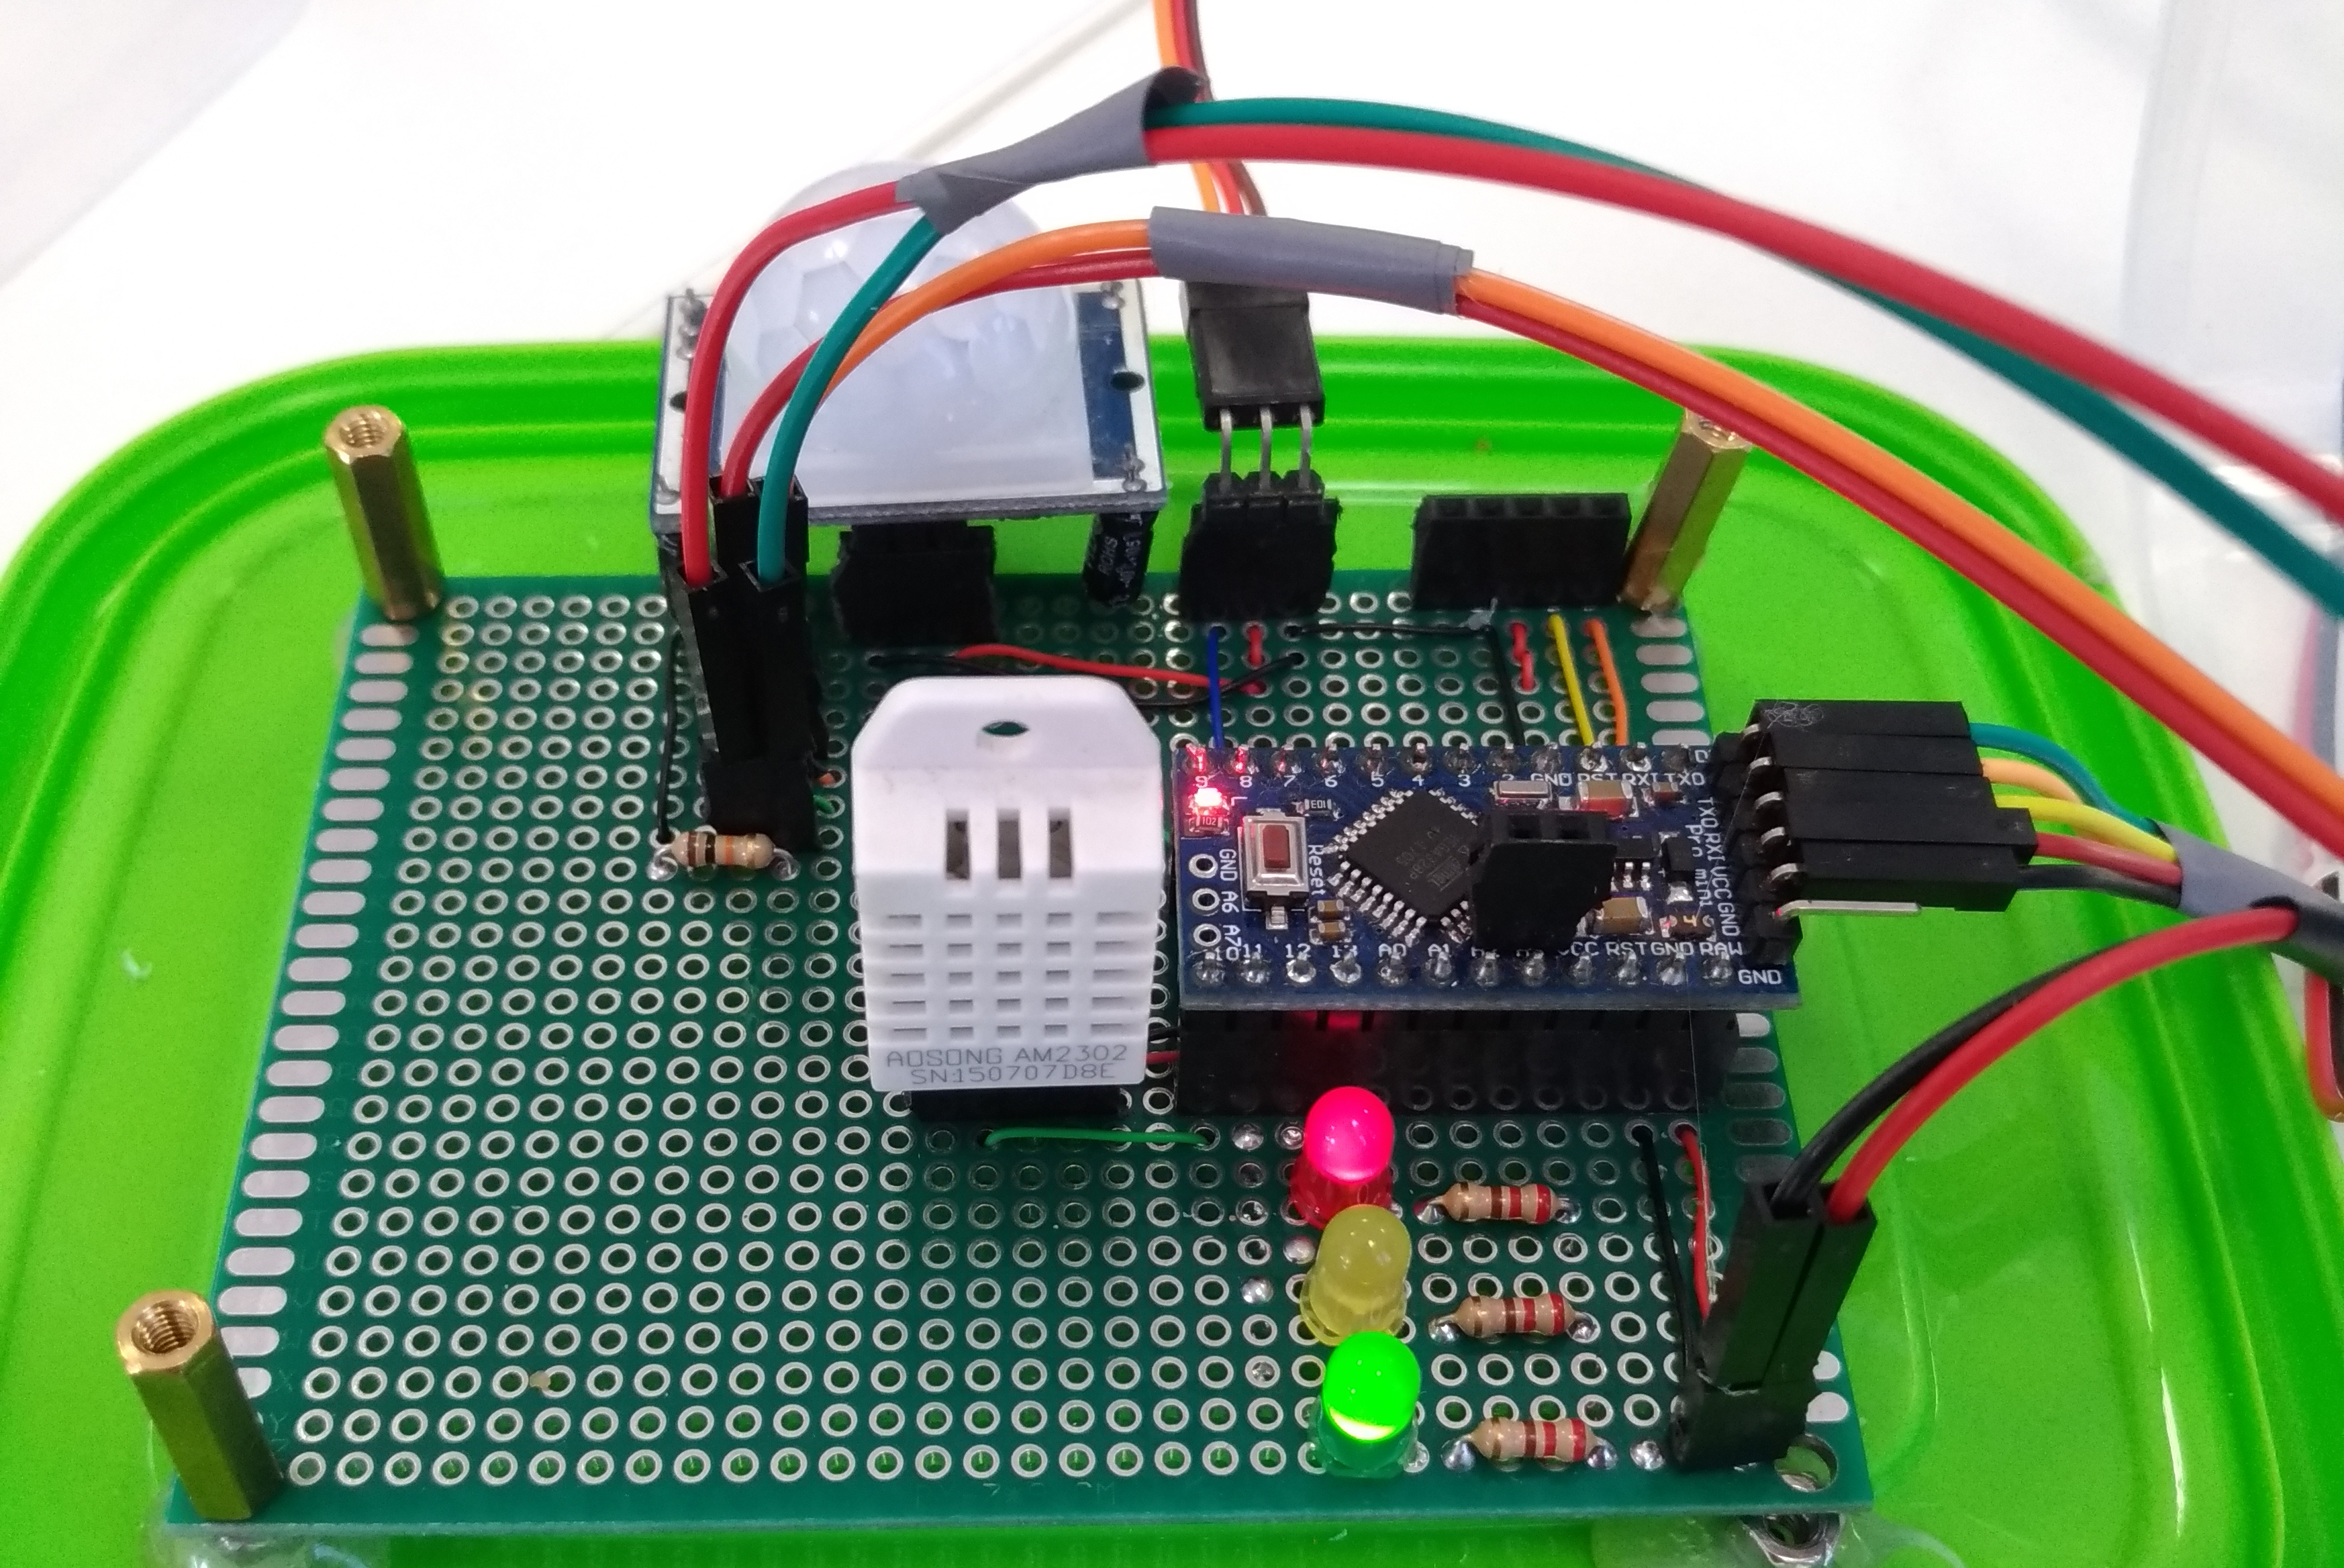
\includegraphics[width=6cm,keepaspectratio]{img/room_board_wiring}
		\caption{Room board wiring}
		\label{fig:room_wiring}
	\end{figure}
	The board is powered by 5V external power attached to the \textit{Raw pin}, this source is shared with the servomotor and the PIR sensor.
	In \ref{fig:room_wiring} is reported a picture of the implementation, in the following table the pins' configuration.
	\begin{center}
		\begin{tabular}{||l | l | l ||} 
			\hline
			Red led 			& 13 & D OUTPUT\\ 
			\hline
			Yellow led 			& 12 & D OUTPUT\\
			\hline
			Green data 			& 11 & D OUTPUT\\ 
			\hline
			DHT data 			& 10 & D INPUT\\ 
			\hline
			PIR data 			& 9 & D INPUT\\ 
			\hline
			ServoMotor PWM 		& 8 & D OUTPUT\\ 
			\hline
			Open Switch 		& 7 & D INPUT\\ 
			\hline
			Closed Switch 		& 6 & D INPUT\\ 
			\hline
			USART TX	 		& 0 & D OUTPUT\\ 
			\hline
			USART RX 			& 1 & D INPUT\\ 
			\hline
		\end{tabular}
	\end{center}
	